\section{Floquet Landau level-like bands in Dirac systems}
In this section we demonstrate a Dirac system in the presence of a standing non-uniform circularly polarized light becomes an effective Dirac Hamiltonian with a magnetic field that is composed of the electric field component of light.
Dirac electrons can be represented with a generic model 2D Hamiltonian honeycomb monolayer in the presence of a gauge potential as

\begin{figure}
  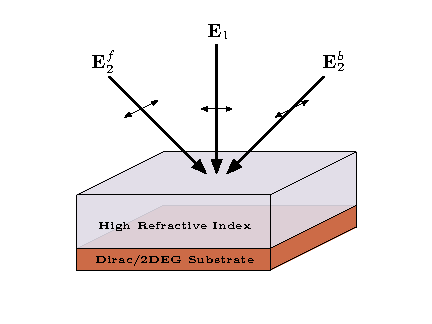
\includegraphics[width=0.5\textwidth]{./figures/fll-setup.pdf}
  \caption{Schematic of two oblique (forward and backward) and one normal incident light on graphene or a 2DEG substrate with high refractive index material on top. Oblique lasers have polarization in $y$-axis and travel in $xz$-plane and normal incidence laser has polarization in the $x$-axis and travel in $yz$-plane. With beam width large enough to cover the device fully.}
  \label{fig:fll-setup}
\end{figure}

\begin{equation}\label{eq:HDirac}
  \ham(t) = v_{F} \bm{\sigma} \cdot \left(\vec{p} + e\vec{A}(t)\right),
\end{equation}
where $\vec{A}$ is the gauge potential, $\vec{p}$ is the momentum operator, $v_F$ is the Fermi velocity of Dirac fermions, $e$ is electron charge, and $\vec{\sigma}$ the Pauli matrices vector in 2D.
The light is made of three linearly polarized laser lights, as shown in Fig. \ref{fig:fll-setup}.
Where the first is normally incident in the $z$-axis with polarization in the $x$-axis.
The second and third are of oblique incidence in the $xz$-plane, to acquire non-uniformity in the $x$-axis, with polarization in the $y$-axis, and mirrored about the $yz$-plane.
This is to introduce $x$-dependence with the $p_y$ term of the Dirac Hamiltonian.
The relevant electric field components at the Dirac system interface are

\begin{align} \label{eq:EDfield}
\vec{E}_{1} &= E\cos \omega t\ \hat{x}, \nonumber \\
\vec{E}_{2} &= \vec{E}_2^f + \vec{E}_2^b = E\sin(Kx)\sin 2\omega t\ \hat{y},
\end{align}
%Where $\omega$ is angular frequency of light with time $t$ and $K=2\pi /d$ with $d$ being the spatial period of the electric field with amplitude $E$.
Where $\omega$ is angular frequency of light with time $t$ and $K = \omega \sin{(\theta_i)} / v_p$, with $\theta_i$ as incident angle of oblique light and $v_p$ is phase velocity of light.
%Notice, the second electric field has twice frequency of the first, this is a requirement to make the Dirac Hamiltonian into a Landau level-like Hamiltonian, the derivation in REFERENCE APPENDIX can inform the reader of this choice.
Notice, the second electric field has twice frequency of the first, this allows for the second gauge potentials $\sigma_y$ to have non-zero commutation with the first gauge potentials $\sigma_x$, and due to the high-frequency expansion used later, allows for the second gauge potential to return to a $\sigma_y$, as seen in \ref{fll-dirac-derivation}.
This form of the electric field relates to the following gauge potential, via $\vec{E} = -\partial_t \vec{A}$ as

\begin{equation}\label{eq:ADirac}
  \vec{A}(t)= \dfrac{E}{\omega} \left\langle -\sin \omega t, \tfrac{1}{2}\sin(Kx) \cos 2\omega t \right\rangle,
\end{equation}%
Substituting Eq.~\eqref{eq:ADirac} into Eq.~\eqref{eq:HDirac}, we arrive at%

\begin{equation}\label{eq:HDtime}
  \ham(t)=\ham_{0} - \sigma _{x} \dfrac{v_F eE}{\omega} \sin {\omega t} - \sigma _{y} \dfrac{v_F eE}{2\omega}\sin{(Kx)} \cos2\omega t,
\end{equation}%
where $\ham_0 = v_{F}\bm{\sigma}\cdot\vec{p}$.
Due to the laser light's time-translation symmetry through $A(t+T)=A(t)$ with $T=2\pi /\omega $, one can apply the Floquet theory \cite{AEE, MBL, supp} and obtain an effective Hamiltonian from Eq.~\eqref{eq:HDtime}.
This introduces the quasienergy matrix $Q_{m,m+n} = H_n + m\hbar\omega\delta_{n0}$ after performing the Fourier time-transform of the Hamiltonian, given as

\begin{equation} \label{eq:fourier-time-transform}
  H_n = \dfrac{1}{T} \int_{0}^{T} \ham(t) e^{-in\omega t} dt,
\end{equation}
then we are left with modes $m=0,\pm1,\pm2$.
To use the high-frequency approximation we require $\hbar\omega \gg H_{\pm1,\pm2}$, the off-diagonal terms.
After applying the high-frequency approximation to first and second order expansion in $\hbar\omega$, it leads to the zeroth-mode effective Hamiltonian in Eq.~\eqref{eq:HDtime} as

\begin{equation} \label{eq:HDeff}
  H_{\text{eff}}= H_{0}-\sigma_y\frac{v_F^3 e^2 E^2 p_y}{\hbar^{2}\omega^{4}}
  +\sigma_y\frac{v_F^3 e^3 E^{3}\sin{(Kx)}}{4\hbar^{2}\omega^{5}}
  -\sigma_x\frac{v_F^3 e^2 E^2 \left\{p_x, \sin^2{(Kx)} \right\} }{8\hbar^{2}\omega^{4}}.
\end{equation}
The derivation can be found in the Appendix \ref{fll-dirac-derivation}.
In Eq. ~\eqref{eq:HDeff}, the first order term in $\hbar \omega$ leads to gap at the Dirac point in normally incident circularly polarized light experiments \cite{YHW, JWM} and is zero here due to the non-uniformity nature of incident laser lights.
This effective Hamiltonian can be simplified in the long wavelength limit, $Kx \ll 1$ to

\begin{align} \label{eq:HeffDirac}
  %\ham_{\text{eff}} &= v_F \sigma_x p_x + v_F \sigma_y \left[ \left( 1- \dfrac{v_F^2e^2E^2}{\hbar^2\omega^4} \right) p_y + \dfrac{K v_F^2 e^3 E^3}{4 \hbar^2 \omega^5} x \right] \nonumber \\
  \ham_{\text{eff}}^D &= v_{F}\sigma_{x}p_{x}+v_F\sigma_{y} \left( C p_{y} + eB^Dx \right),
\end{align}%
where $C = 1-\left(\tfrac{v_{F}eE}{\hbar\omega^2}\right)^2$ and $B^D=\frac{Kv_F^2 e^2E^3}{4\hbar^{2}\omega^{5}}$.
In accordance with Eqs.~\eqref{eq:HDeff} and ~\eqref{eq:HeffDirac}, there is least anisotropy in the Dirac spectrum in addition to zero gap.
Diagonalizing the Hamiltonian in Eq.~\eqref{eq:HeffDirac}, we obtained the eigenvalues for Dirac system as%

\begin{equation} \label{eq:DiracEner}
  \epsilon_{n}^D = \pm v_F^2 \sqrt{\dfrac{nK e^3 E^3}{2 \hbar \omega^5}}
\end{equation}
which is similar to graphene LLs spectrum in the limit of equal velocities.
The effective magnetic field in the Dirac Hamiltonian achieves a highly degenerate energy spectrum similar to LLs.
From a classical point of view we call this a LL-like spectrum, the difference being electrons are not necessarily in cyclotron orbits but orbits, potentially more complicated, due to CPL producing a Coulumb force in the material's 2D plane.

There are several ways to enhance the effective magnetic field and directly LL-like energies for a Dirac system.
Electric field strength can be increased within reason as we are limited by the photon energy to ensure the high-frequency expansion holds, $E \ll 2\hbar\omega^2/e v_F$, one can reasonably use electric field strengths up to 20\% of the limit due to photon energy.
The lights wavenumber $K= \omega \sin{(\theta_i)} / v_p$ has a linear relationship to photon energy, too.
Overall, considering the high-frequency limit on the electric field, the effective field $B^D \propto \omega^2 \sin{(\theta_i)} / (v_F v_p)$.
Increasing photon energy is one way to enhance the effective magnetic field.
As considered in previous literature, when photon energy and electric field are increased more energy is pumped into the system, shorter pulses are required to prevent damaging the system \cite{YHW, JWM}.
Without too much consequence the incident angle can be increased up to $\pi/2$ and descreasing the phase velocity of light would enhance the effective magnetic field.

%\Blue{This next paragraph should be in the discussion since it uses similar language and results as 2DEG?}
%It is important to note, that this system experiences QHE for values of $C\neq0$ and can flip chirality when $C$ changes sign, more details in REFERENCE APPENDIX.
%We can have gapped Dirac spectrum and QAHE by using uniform circularly polarized laser light as observed in experiments \cite{YHW, JWM} or by using any substrate like hBN.
%Now, we have shown one can achieve a highly degenerate Landau level-like spectrum and QHE with an effective magnetic field strength which is directly proportional to third order of the electric field and inversely proportional to the product of spatial period and fifth order of the frequency of the polarized light $\propto (E^3/(d\omega^5))$.
%This factor of the laser lights can be tuned and thus effective magnetic field can be enhanced in such nonequilibrium systems.
%In the case of uniform circularly polarized light, one can imagine the Coulomb force makes the charged particles move in a cyclotron orbit.
%In constrast, for non-uniform circularly polarized light, charged particles are not necessarily in cyclotron orbits but in some form of closed orbit preventing the charged particles from moving on average in a given direction, hence we define them as Landau level-lik.
